\section{Komponente des Embedded Linux Betriebssystems für ARM Prozessoren}
\label{cha:tech_grund:sec:Komponente_eines_Emb_Lin_Sys}
In diesem Abschnitt möchte ich auf die wesentlichen Komponenten von eingebetteten Linux-Betriebssystems im Detail eingehen. Im Anschluss daran wird der typische Boot-Prozess solcher Systeme beschrieben.
Ein auf Linux basierendes Betriebssystem wird in Form einer Linux-Distribution angeboten. Es handelt sich dabei um eine Sammlung von Softwarepaketen, Bibliotheken und Dienstprogrammen zusammen mit einer eigenen Linux-Kernel-Variante, die für eine bestimmte Prozessorarchitektur angepasst oder verändert wird. 
Zum Booten eines Linux-Betriebssystems auf einem ARM-Prozessor werden die folgenden Komponenten benötigt:

\begin{itemize}
	\item \textbf{der Bootloader} 
	\item \textbf{Der Gerätebaum(Device-tree)}:
	\item \textbf{Der Linux Kernel}
	\item \textbf{Root filesystem}: beinhaltet die Bibliotheken und Programme, die ausgeführt werden, sobald der Kernel seine Initialisierung abgeschlossen hat.
	\item \textbf{Der \grqq Init\grqq\ Prozess}:
\end{itemize}

\subsection{Der Bootloader}
\cite{Dervis2013}Der Bootloader ist die Software, die beim Einschalten des Systems ausgeführt wird und für das Laden eines Betriebssystems für die Hardware verantwortlich ist. Beim Einschalten des Rechners, auf denen Linux als Betriebssystem installiert ist, wird nach der ersten Einrichtung der Bootloader, der für die Initialisierung der Hardware-Peripherie und das Laden des Bitstreams im FPGA verantwortlich ist, in den Speicher geladen und der Code ausgeführt.\\
Der Bootloader muss zunächst von der Festplatte in den Prozessorspeicher geladen werden, bevor er ausgeführt werden kann. Beim Zynq UltraScale+MPSoC wird UBoot zum Laden des Linux-Kernels verwendet, und die Bootload-Phase ist hier in zwei Stufen unterteilt: die FSBL-Phase und die U-Boot-Phase

\subsection{Device-tree}
\begin{figure}[h]
	\begin{center}
		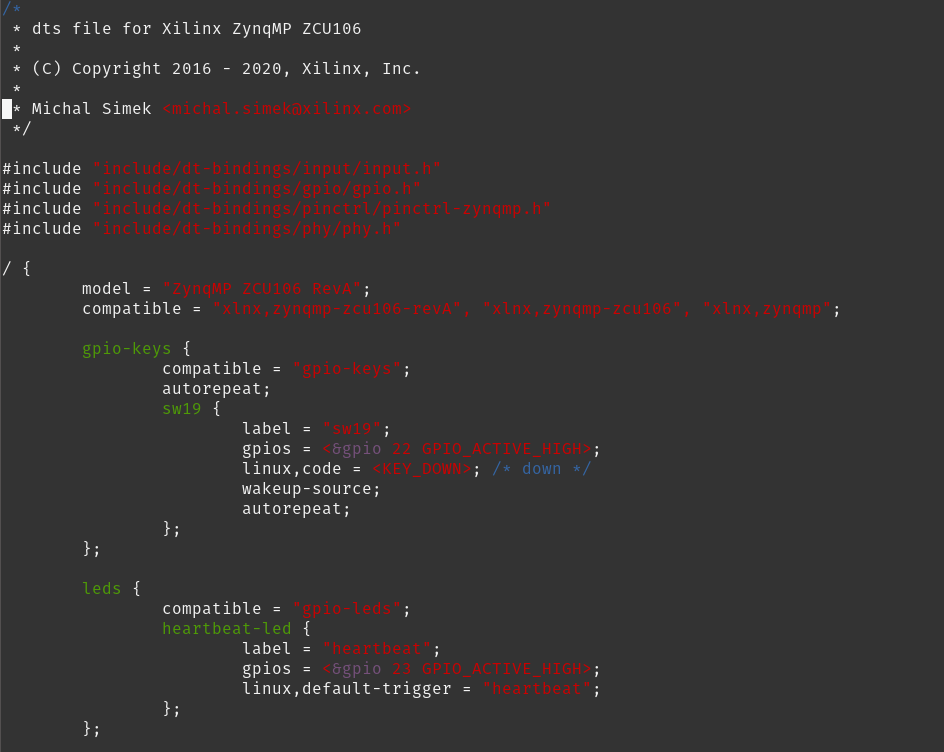
\includegraphics[width=1\textwidth]{./images/device-tree.jpg}
	\end{center}
	\vspace{-5pt}
	\caption[ZCU106-Gerätbaum gpio-keys and leds]{Ein Screenshot des ZCU106-Gerätebaums, der den Inhalt des gpio-keys und leds  auf dem Board zeigt} % Eckige Klammer (optional): Caption-Text in Abbildungsverzeichnis
	\label{fig:device:tree}
	\vspace{-5pt}
\end{figure}	
Die Abbildung ~\ref{fig:device:tree} zeigt Informationen zu den Schalter- und led-Knoten im Device Tree des Xilinx ZCU106 Boards. Hier wird z.B. angegeben, an welchem gpio-Pin der Schalter SW9 auf der Platine angeschlossen ist.\\
\cite{Dervis2013}Der Linux-Kernel benötigt Informationen über den Prozessor, auf dem er ausgeführt wird, die Peripheriegeräte, mit denen der Prozessor verbunden ist, ihre Schnittstellen zum Prozessor und ihre physikalischen Adressen. Der Kernel muss zur Initialisierung der Treiber und der mit diesen Peripheriegeräten verbundenen Dienste auch überprüfen, dass die Funktionen, die in seiner Konfiguration aktiviert wurden, tatsächlich von der Hardware unterstützt werden, die er steuert. Dabei kann es sich um Informationen über die Taktgeber und Register der Hardware oder über die mit der Hardware verbundenen Peripheriegeräte wie den externen Speicher, SPI handeln.\\

Der Zynq UltraScale+MPSoC verwendet daher den Device-Tree, um die Geräte- und Peripherie-Informationen wie physikalische Geräteadressen, E/A-Registeradressen, Speicheradressraum und Interrupt-Informationen während des Bootvorgangs an den Kernel weiterzugeben.\\
Der Gerätebaum wird im Textformat in einer Datei mit der Erweiterung \ ".dts"\ dargestellt. Hierbei handelt es sich um eine Quelltextdatei, die Informationen über Geräte und Verbindungsbusse beschreibt, die mit einer Computer-Hardware verbunden sind. Sie ist in Form von \ "Knoten"\ organisiert, deren Stammverzeichnis durch \grqq /\grqq\ dargestellt wird, genau wie im Linux-Stammdateisystem. Jeder Knoten hat einen Namen, der ein mit dem Prozessor verbundenes Gerät oder einen Bus darstellt, und der Knoten besteht aus Eigenschaften. Jeder übergeordnete Knoten für ein bestimmtes Peripheriegerät oder einen Bus kann \ "Kind"\ -Knoten für Geräte enthalten, die mit diesem Peripheriegerät oder Bus verbunden sind. Die Werte der Eigenschaften können Zeichenketten oder Listen von Zeichenketten sein, oder sie können leer sein, wenn das Vorhandensein oder Nichtvorhandensein des Wertes eine boolesche Logik an den Kernel übermittelt. Die Device-Tree-Quelldatei wird mit Hilfe des \ "dtc -Compilers"\ zu einem Device-Tree-Blob (.dtb) kompiliert.

\subsection{Der Linux Kernel}
Das ist das Herzstück des Systems, das die Systemressourcen und Schnittstelle zur Hardware verwaltet. Die Hauptfunktionen des Linux-Kernels sind die folgenden~\cite{linuxkernel.}:
\begin{itemize}
	\item Planung von Prozessen und Einrichten einer Umgebung für ihre Ausführung.
	\item  Zuteilung von Speicher an einen Prozess und Schutz des von einem Prozess verwendeten Speichers vor anderen Prozessen.
	\item \ Verwaltung der Kommunikation zwischen den Prozessen, um eine effiziente Ausführung der Prozesse zu gewährleisten
	\item Sicherstellung der Integrität des Systems, wenn das Computersystem mehrere Benutzer hat, die berechtigt sind, Änderungen am Root-Dateisystem und an Softwarepaketen vorzunehmen.	
	\item Verwalten der Computerressourcen und des Zugriffs auf diese Ressourcen
\end{itemize}

Nachdem der Bootloader den Gerätebaum und den Kernel in den DRAM des Prozessors geladen hat, teilt er dem Kernel die Adresse des Gerätebaums mit, bevor der Kernel mit der Ausführung beginnt. Der Kernel prüft dann der Reihe nach alle Hardware-Peripheriegeräte, Clock-Generator und Speicher, die vom FSBL initialisiert wurden, und aktiviert dann alle mit der zugrunde liegenden Hardware verbundenen Dienste und Funktionen, die in der Kernelkonfiguration aktiviert wurden. Sobald der Kernel mit diesen Aufgaben fertig ist, hängt er das Root-Dateisystem ein und führt den "init"-Prozess aus, der es dem Benutzer ermöglicht, in den Benutzerraum einzutreten.

\subsection{Das Linux Root files System (Rootfs)}

Das Linux-Root-Dateisystem [\cite{Dervis2013}] enthält alle binären ausführbaren Dateien, Geräteinformationen, Prozessprotokolle, Softwarepakete und Bibliotheken, die vom Benutzer in seinem Benutzerbereich benötigt werden, um das Linux-Betriebssystem effizient zu nutzen. Das Dateisystem auf der Festplatte ist in Verzeichnissen organisiert. Das Root-Dateisystem wird in das Verzeichnis\grqq /\grqq\ des Dateisystems eingehängt, welches die Spitze der Hierarchie des Root-Dateisystems markiert.

\subsection{Der Init Prozess}

Der "init"-Prozess [\cite{Dervis2013}] wird als erster Prozess im Benutzerbereich vom Kernel initiiert und ist für die Initialisierung der Systemverwaltungsdienste zuständig, bevor die Benutzer sich anmelden können. Alle Software-Dienste, die im Root-Dateisystem installiert und im Benutzerraum aktiviert wurden, werden vom "init"-Prozess ausgeführt, bevor sich die Benutzer sich am System anmelden

Als Nächstes wird den Boot-Prozess bei Systemen, die auf Zynq UltraScale+ MPSoCs basiert sind, erläutert, da dies genau die Plattform ist, die wir für unsere Arbeit verwenden werden.

\subsection{Der Zynq UltraScale+MPSoC Boot-Prozess}

Zum Booten von Linux auf dem Zynq UltraScale+MPSoC muss das Boot-Image (BOOT.BIN) auf dem Boot-Medium entsprechend dem vom Benutzer gewählten Boot-Modus vorhanden sein [\cite{Xilinx2017}[p.~14]]. Das ZCU106 Board unterstützt das Booten über JTAG, Quad-SPI Flash, SD Card und NAND Flash Drive. In dieser Arbeit booten wir Linux von der SD-Karte[\cite{Xilinx2020}[p.~61]], daher muss die Datei BOOT.BIN auf der FAT32-Partition der SD-Karte vorhanden sein. Die BOOT.BIN-Datei wurde so konfiguriert, dass sie die Platform Management Unit Firmware (PMUFW), die FSBL und die ausführbaren U-Boot-Dateien beinhaltet, welche die empfohlene Konfiguration für den Zynq UltraScale+ ist. Die BOOT.BIN enthält in dieser Arbeit auch den FPGA-Bitstream zur Programmierung der programmierbaren Logik (PL). Für ein vollständiges Booten über eine SD-Karte sollten das Kernel-Image (Image) und der Device-Tree-Blob ("Projektname.dtb") ebenfalls auf der FAT32-Partition vorhanden sein. Das Root-Dateisystem muss auf der EXT4-Partition der SD-Karte vorhanden sein.\\
Der Bootvorgang von Linux auf dem Xilinx Zynq UltraScale+MPSoC lässt sich in vier Phasen unterteilen

\begin{itemize}
	\item Die Boot-Setup-Phase
	\item Die Bootloader-Phase
	\item Die Kernel-Boot-Phase
	\item und Die \grqq init\grqq-Phase
\end{itemize}

\subsubsection{Die Boot-Setup-Phase}
\label{cha:tech_grund:sec:Komponente_eines_Emb_Lin_Sys:sub:sec:pmu}
Die Platform Management Unit (PMU) und die Configuration Security Unit (CSU) sind für das Einrichten des Zynq UltraScale+ MPSoC verantwortlich, bevor Linux auf dem PS gebootet werden kann . Die Boot-Setup-Phase besteht aus drei Phasen, die wie folgt unterteilt werden können[\cite{XilinxInc.2019}[p.~27]]:
\begin{itemize}
	\item \textbf{Pre-configuration stage (Oder Vor-Konfigurationsphase)}: Dieser Phase wird von der PMU angesteuert, die den PMU-ROM-Code(PBR). Nachdem der PBR-Code ausgeführt wurde, übergibt er die Systemkontrolle an die Configuration Security Unit (CSU). Die wichtigsten Schritte der Vor-Konfigurationsphase sind im Folgenden aufgeführt[\cite{XilinxInc.2019}[p.~57]]:
	\begin{itemize}
		\item Initialisieren des Systemmonitors
		\item Initialisierung der Phase Locked Loops (PLL) für Takte
		\item Leeren des PMU-RAMs.
		\item Initialisieren Sie des Dynamic Random Access Memory (DRAM).
		\item Freigabe der CSU oder Eintritt in den Fehlerzustand.
	\end{itemize}
	\item \textbf{Configuration stage oder (Konfiguration der Phase)}:Diese Phase übernimmt das Laden des First-Stage-Bootloader-Codes (FSBL) für den PS in das On-Chip-RAM (OCM), und zwar sowohl im sicheren als auch im unsicheren Boot-Modus. Während des Bootvorgangs lädt die CSU auch die PMU-Benutzerfirmware (PMU FW) in das PMU-RAM, um in Verbindung mit dem PMU-ROM Plattform-Management-Dienste bereitzustellen.
	\item \textbf{Post-configuration stage oder (Post-Konfigurationsphase)}: Nach dem Start der FSBL-Ausführung geht der CSU-ROM-Code in die Post-Konfigurationsphase über, die für die Reaktion auf Systemmanipulationen verantwortlich ist
\end{itemize}

\subsubsection{Die Bootloader-Phase}
\label{cha:tech_grund:sec:Komponente_eines_Emb_Lin_Sys:sub:sec:fsbl}
\textbf{\normalsize First Stage Bootloader (FSBL)}\\
Die FSBL ist der sekundäre Programmlader in der Terminologie des generischen ARM-Prozessor-Boot-Prozesses. Der FSBL führt die folgenden Aufgaben aus. FSBL führt die folgenden Aufgaben aus[\cite{XilinxInc.2019}]
\begin{itemize}
	\item Suchen in der FAT32-Bootpartition der SD-Karte nach dem PL-Bitstream und dem second stage Bootloader (das U-boot).
	\item Initialisierung der PS-Hardware, der E/A-Geräte, des Speichers und der Takte entsprechend der Konfiguration, die durch das in der Xilinx Vivado Design Suite spezifizierte Hardware-Design definiert ist
	\item Programmieren des PL mit dem FPGA-Bitstream
	\item Laden der ARM Trusted Firmware (ATF) und das U-Boot in den APU-Prozessorspeicher.
\end{itemize}

\textbf{\normalsize Das U-boot}\\
Wenn der Prozessor eingeschaltet wird, enthält der Prozessorspeicher kein Betriebssystem, sodass ein Bootloader erforderlich ist, um den Linux-Kernel und den Gerätebaum aus dem Speicher in den Prozessorspeicher zu laden, diese Aufgabe wird also vom U-boot Übernomen. Der U-Boot ist der Second Stage Bootloader (SSBL) für den Xilinx Zynq UltraScale+ MPSoC oder der Tertiary Program Loader (TPL) in der Terminologie des generischen ARM-Bootprozesses.  U-Boot kann den Kernel und den Device-Tree über das Netzwerk mittels Ethernet, über JTAG, von der SD-Karte, Quad-SPI-Flash und vom NAND-Flash-Laufwerk laden.

Die Abbildung ~\ref{fig:boot:process} Es zeigt die Rolle der verschiedenen Einheiten des Zynq UltraScale+MPSoC beim Booten des Linux-Betriebssystems auf der Hardware. Man sieht, dass die PMU die CSU freigibt, die wiederum die FSBL lädt. Die FSBL lädt dann das ATF und das U-Boot. Das U-Boot ist dann für das Booten von Linux auf der Hardware verantwortlich.

\begin{figure}[h]
	\begin{center}
		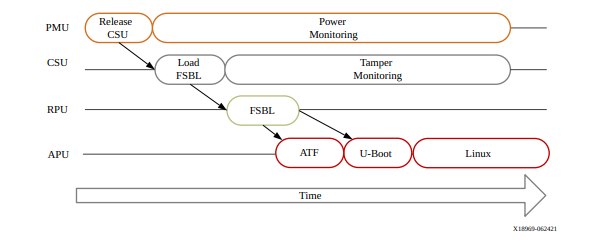
\includegraphics[width=1.1\textwidth]{./images/boot-flow.jpg}
	\end{center}
	\vspace{-5pt}
	\caption[der Bootvorgang bei zynq+MPSoCs]{Überblick über den Bootvorgang \cite{XilinxInc.2019}[p.~58]} % Eckige Klammer (optional): Caption-Text in Abbildungsverzeichnis
	\label{fig:boot:process}
	\vspace{-5pt}
\end{figure}


\subsubsection{Der Boot Flow}

Der Zynq UltraScale+ MPSoC kann in zwei Modi gebootet werden: im sicheren und im unsicheren Modus. Diese werden im Folgenden beschrieben[\cite{XilinxInc.2019}[p.~58]]

\textbf{\normalsize \textit{Nicht gesicherter Bootvorgang}}\\
In diesem Boot-Modus gibt die PMU die CSU frei und wechselt in den Servicemodus, in dem sie die Plattform überwacht. Die CSU lädt die FSBL in den On-Chip-Speicher (OCM) der APU und die PMUFW in das RAM der PMU. Die PMUFW wird parallel zur Ausführung der FSBL ausgeführt und läuft, bis Linux auf dem Zynq UltraScale+ MPSoC gebootet ist. Der FSBL initialisiert die Peripheriegeräte, E/A-Geräte, den Speicher und die Takte und übergibt sie an den ATF, der sie dann an das U-Boot weitergibt. Das U-Boot lädt dann den Linux-Kernel in das APU-Prozessor-Memo

\textbf{\normalsize \textit{gesicherter Bootvorgang}}\\
Der sichere Bootvorgang unterscheidet sich vom unsicheren Bootvorgang nur durch einige zusätzliche Authentifizierungs- und Entschlüsselungsschritte, die von der CSU ausgeführt werden. Beim sicheren Bootvorgang gibt die PMU den Reset der Configuration Security Unit (CSU) frei und geht in den PMU-Servermodus über, in dem sie die Stromversorgung überwacht. Nachdem die PMU das Zurücksetzen der CSU aufgehoben hat, prüft die CSU, ob eine Authentifizierung durch die FSBL oder die Benutzeranwendung erforderlich ist 

\subsection{Die Kernel-Boot-Phase}
Das U-Boot sorgt für das Laden des Kernel-Images und des Gerätebaums in den Speicher des APU-Prozessors und die Übergabe der Kontrolle an den Kernel. Der Kernel erhält auch die Adresse des Gerätebaums, der den Kernel über die Hardware-Peripherie, E/A-Geräte, Speicher und Taktgeber informiert. Basierend auf diesen Informationen startet der Kernel den Bootvorgang und aktiviert die Treiber und Dienste, für die der Kernel konfiguriert wurde. Nachdem der Kernel gebootet hat, mountet er das Root-Dateisystem entsprechend den an den Kernel übergebenen Boot-Argumenten. Je nach dem an den Kernel übergebenen Boot-Argument hängt der Kernel das Root-Dateisystem über NFS oder von der SD-Karte oder einem anderen permanenten Speicherort ein.

\subsection{Die init-Phase}

Nach Einhängen des Root-Dateisystems sucht der Kernel nach der ausführbaren Datei des für die Linux-Distribution angegebenen init-Prozesses. Sobald der Kernel den init-Prozess gefunden hat, führt er ihn aus und übergibt die Kontrolle an den init-Prozess. Der init-Prozess aktiviert dann alle Systemverwaltungs- und andere Hintergrunddienste, die im Root-Dateisystem installiert und im Benutzerbereich aktiviert wurden. Nach der Aktivierung dieser Dienste startet der init-Prozess den Benutzeranmeldungsprozess, der es dem Benutzer ermöglicht, den Benutzerraum zu betreten\\
Alle bisher genannten Linux-Komponenten, ob der Bootloader, der Kernel oder das Root-Dateisystem können mit einem Build-System wie dem Yocto-Projekt erstellt werden. Da unser FPGA aber einen MPsoc enthält, der einen Bootloader, ATF-Firmware, pmufw, den Bitstream und u-boot benötigt, ist ein Build System zu verwenden, das automatisch alle diese Komponenten erzeugen kann.. Hierfür ist Petalinux am besten geeignet. Im nächsten Abschnitt werde ich das Petalinux Build System vorstellen. 


